\documentclass{ccn}

\addbibresource{ccn_references.bib}

\title{Tracing Sparse Feature Circuits in Vision Transformers}

% \author{Zirui Hu \\
%   Department of Physics, Brown University}

\begin{document}

\maketitle

\begin{abstract}
This work implements a pipeline for cross-layer circuit analysis in Vision Transformers (ViTs), combining sparse feature learning, candidate filtering, relation analysis, and intervention-based tests. Sparse autoencoders are trained on intermediate activations, candidate units are filtered using statistical and visual criteria, and retained units are analyzed through cross-layer consistency, feature-to-output edge strength, preliminary feature-to-feature relations, and targeted interventions. The current results already produce units and local structures that can be used for early circuit analysis in ViTs, and provide a workable basis for broader cross-layer circuit reconstruction.
\end{abstract}

\section{Introduction}

Recent work in large language models has shown that intermediate computational structure can be studied through sparse features, attribution patterns, and interactions between internal units \citep{Ameisen2025CircuitTracing,Marks2024SparseFeatureCircuits,Templeton2024ScalingMonosemanticity}. These developments provide useful methodological inspiration for vision models. Vision Transformers (ViTs) are a natural setting for this problem because they process structured visual inputs through repeated attention and token mixing, suggesting that meaningful computation may be distributed across depth rather than localized to a single layer \citep{Dosovitskiy2020ViT}.

The goal of this work is to build a practical pipeline for circuit analysis in ViTs. In this setting, sparse intermediate units serve as an intermediate representation on top of which cross-layer relations and interventions can be analyzed more systematically. The project uses this sparse intermediate basis to support circuit recovery. The current workflow includes candidate unit discovery, feature-to-output analysis, feature-to-feature analysis, and cross-layer local structure analysis.

\section{Sparse Feature Pipeline}

Sparse autoencoders (SAEs) are trained on selected intermediate activations of a ViT \citep{Marks2024SparseFeatureCircuits,Templeton2024ScalingMonosemanticity}. In the current version, the analysis focuses on attention-output representations. A broader multi-stream setup was initially explored, and at the present stage that configuration was less stable. The analysis was therefore temporarily narrowed to attention-output activations because they were easier to train and validate and provided a more reliable basis for the rest of the pipeline. This narrowing is a practical choice for the current stage rather than a fixed limitation, and broader representations may be revisited once the pipeline is further stabilized.

Candidate units are filtered using activation coverage, spike-like behavior, top-activating examples, and class-conditional response statistics. These criteria are combined into a feature score that is used to rank and retain units for later analysis. This step retains units that are more stable and visually coherent, so that relation analysis is based on a cleaner set of candidates. In practice, this stage matters because raw high-activation candidates are often too mixed or unstable to support circuit-level interpretation.

Once a filtered set of units is obtained, it is used for circuit-oriented analysis. The analysis examines whether the same unit shows similar visual selectivity across layers, measures feature-to-output edge strength, estimates preliminary feature-to-feature relations, and performs targeted interventions to test whether selected units produce repeatable downstream effects. Sparse feature learning, filtering, relation analysis, and intervention therefore operate as parts of a single pipeline for tracing cross-layer structure \citep{Ameisen2025CircuitTracing,Marks2024SparseFeatureCircuits}.

\section{Preliminary Results}

The current pipeline produces units and relations that can be used for preliminary cross-layer circuit analysis. The current outputs include retained sparse units, feature-to-output relations, preliminary feature-to-feature structure, and targeted intervention results on selected components.

\begin{figure}[!t]
    \centering
    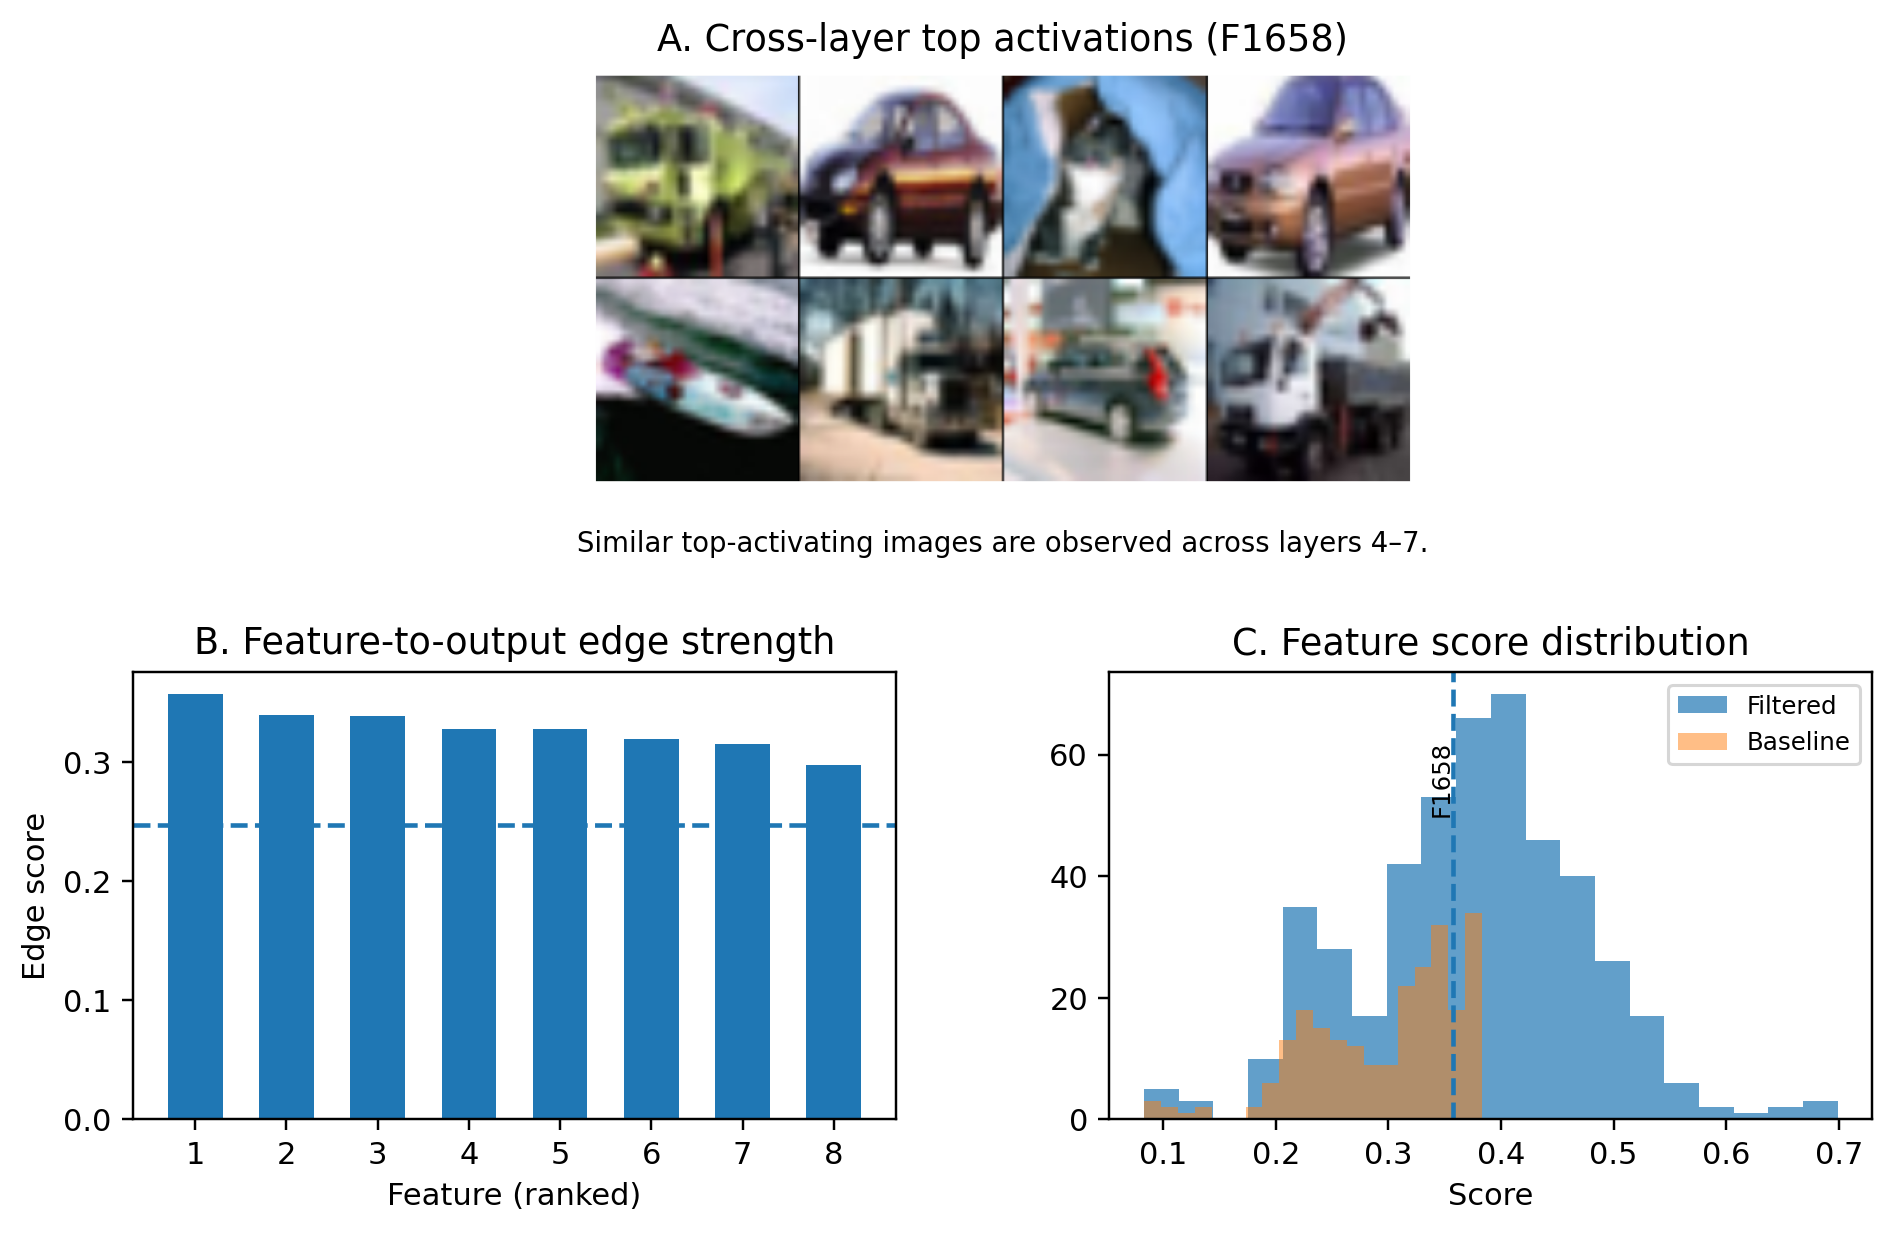
\includegraphics[width=\linewidth]{ccn_split_figure1.png}
    \caption{
    A representative retained unit from the analysis pipeline.
    (\textbf{A}) Feature F1658 shows similar top-activating images across layers 4--7.
    (\textbf{B}) The strongest retained units have higher feature-to-output edge scores than the average level.
    (\textbf{C}) F1658 lies in the upper part of the feature score distribution.
    }
    \label{fig:main_result}
\end{figure}

Figure~\ref{fig:main_result} shows one representative example. Panel A indicates that feature F1658 recurs as a similar visual pattern across layers 4--7. Panel B shows that the strongest retained units also have larger feature-to-output edge scores. Panel C places F1658 in the higher-score region of the retained feature distribution, indicating that it is one of the stronger units in the current run.

The current outputs contain cross-layer visual consistency, output-related relations, preliminary feature-level organization, and intervention-based tests of selected components. These results show local structures that can be used for circuit analysis. The recovered structures are not yet complex, complete, or fully reliable. The current results are best described as an initial cross-layer scaffold, and they already show that the pipeline is producing more than isolated features.

\begin{figure}[!t]
    \centering
    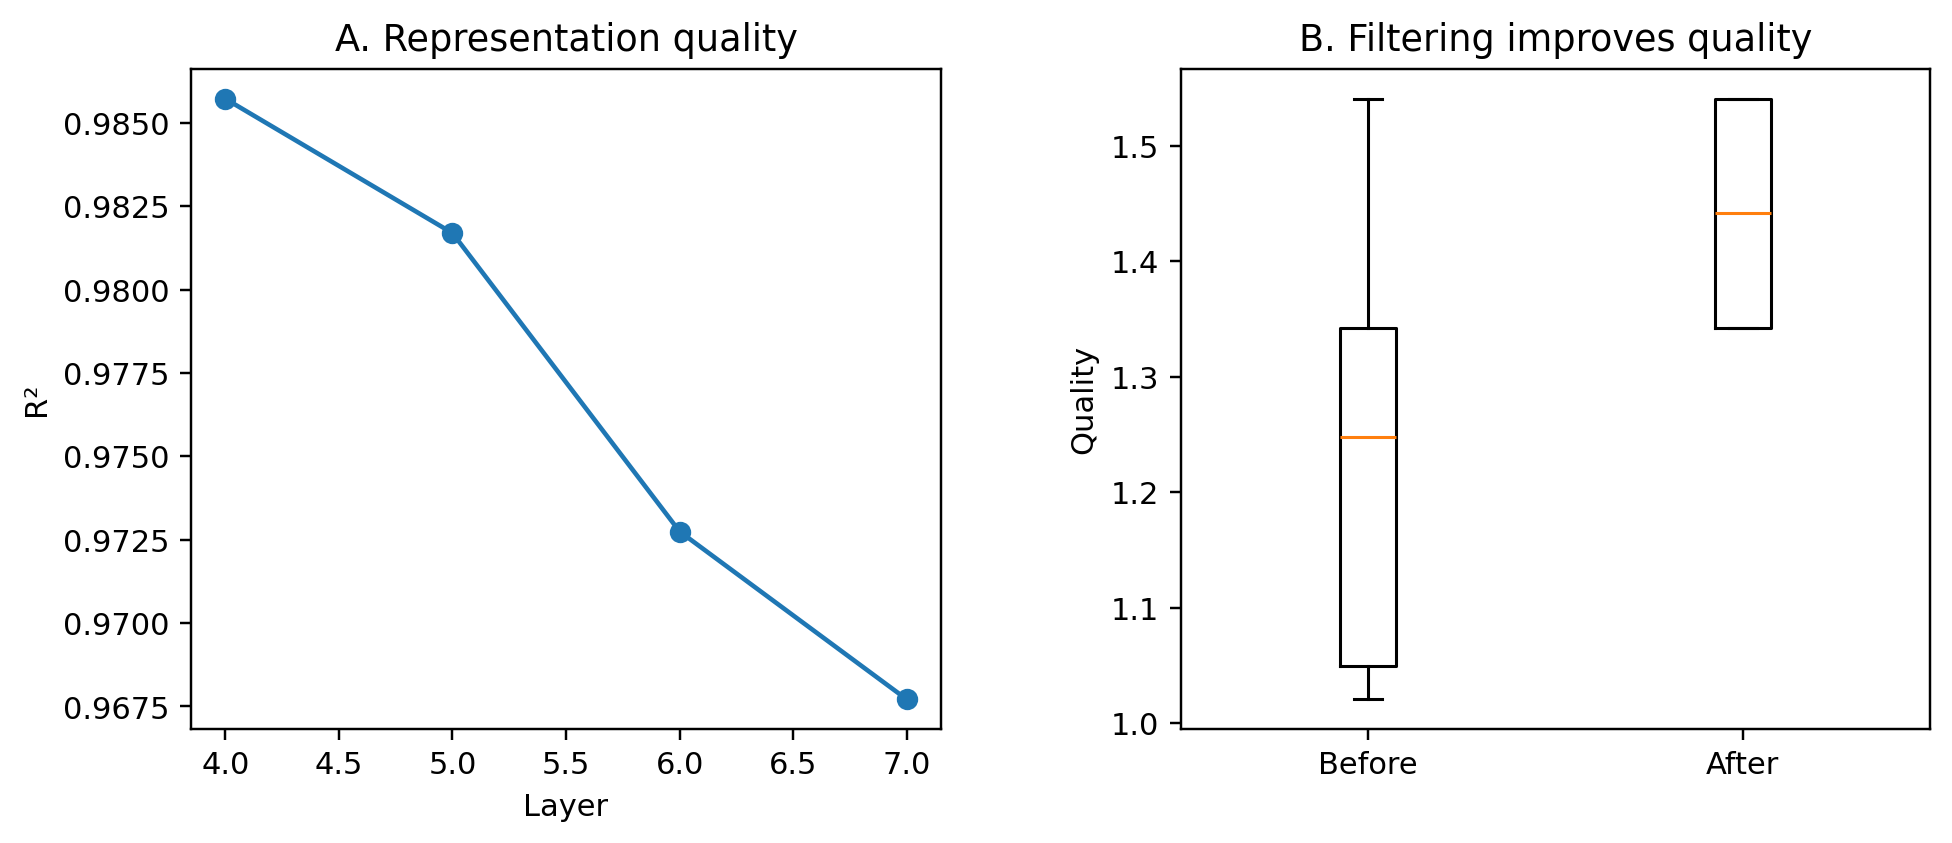
\includegraphics[width=\linewidth]{ccn_split_figure2.png}
    \caption{Two summary statistics of the current pipeline.}
    \label{fig:pipeline_effect}
\end{figure}

Figure~\ref{fig:pipeline_effect} summarizes two additional properties of the pipeline. In panel A, representation quality is measured by SAE reconstruction $R^2$, which remains high across the analyzed layers. In panel B, quality refers to the combined feature score used during filtering, and the boxplots summarize its distribution before and after filtering; the center line indicates the median. These results show that the pipeline selects visually cleaner examples and produces a more suitable basis for later circuit analysis.

\section{Cross-Layer Circuit Analysis}

The present implementation already contains several components needed for broader circuit recovery. It identifies retained sparse units, estimates feature-to-output relations, organizes preliminary feature-to-feature structure, and tests selected components through targeted interventions. The current work continues to extend these local structures within the same framework.

The current work expands the coverage of robust candidate units across more layers, improves the informativeness of intervention tests, and integrates existing feature-to-output and feature-to-feature statistics into more coherent cross-layer subgraphs that can be tested more directly. These relations can already be estimated and partially organized. The current task is to extend them into larger structures that are easier to interpret and more reliable as circuit descriptions \citep{Ameisen2025CircuitTracing,Marks2024SparseFeatureCircuits}.

The present stage can be viewed as an active process of circuit reconstruction in which the pipeline already produces the ingredients of cross-layer structure and continues to assemble them into broader circuits. The immediate work centers on coverage, validation, and integration so that these local results can be expanded into more complete cross-layer circuits.

\section{Discussion}

This work develops a pipeline for cross-layer circuit analysis in ViTs by combining sparse intermediate representations, candidate filtering, relation analysis, and interventions. The current results do not yet provide a complete mechanistic account of ViT computation, but they already recover local circuit structure that can support further analysis. The present outputs show that this is a workable direction for moving from isolated units toward broader circuit structure in vision models.

\printbibliography

\end{document}